% Copyright (c) 2010 Vincent Renaudineau, Jérémie DECOCK

% This document is provided under the terms of the "Creative Commons BY-SA" license.
% For more details, read "legalcode.html" enclosed file or "http://creativecommons.org/licenses/by-sa/2.0/fr/" web page.

\documentclass{beamer}

\usepackage[utf8]{inputenc}
\usepackage[frenchb]{babel}

\usepackage{subfigure}

\mode<presentation> {
    \usetheme{Frankfurt}
}

\usepackage{verbatim}

%\setbeamertemplate{footline}
%{%
%    \leavevmode%
%    \hbox{\begin{beamercolorbox}[wd=.5\paperwidth,ht=2.5ex,dp=1.125ex,leftskip=.3cm plus1fill,rightskip=.3cm]{author in head/foot}%
%    \usebeamerfont{author in head/foot}\insertshortauthor
%    \end{beamercolorbox}%
%    \begin{beamercolorbox}[wd=.5\paperwidth,ht=2.5ex,dp=1.125ex,leftskip=.3cm,rightskip=.3cm plus1fil]{title in head/foot}%
%    \usebeamerfont{title in head/foot}\insertshorttitle\hfill \insertpagenumber{} / \inserttotalframenumber
%    \end{beamercolorbox}}%
%    \vskip0pt%
%}

\title{Exploiting Open-Endedness to Solve Problems Through the Search for Novelty}
\subtitle{[Lehman and Stanley, 2008]}
\author{Jérémie~\bsc{Decock} \and Vincent~\bsc{Renaudineau}}
\institute{UPMC}
\date{24 mars 2010}

\begin{document}

\begin{frame}
\titlepage
\end{frame}

%%%%%%%%%%%%%%%%%%%%%%%%%%%%%%%%%%%%%%%

\begin{frame}
\frametitle{Plan}
%\tableofcontents
\tableofcontents[sectionstyle=show/show,subsectionstyle=hide/hide/hide]
\end{frame}

%%%%%%%%%%%%%%%%%%%%%%%%%%%%%%%%%%%%%%%

\section{Introduction}
\begin{frame}
\begin{center}
{\LARGE Introduction}
\end{center}
\end{frame}

\subsection{Introduction}

\begin{frame}{Introduction}
    Exploiting Open-Endedness to Solve Problems Through the Search for Novelty [Lehman and Stanley, 2008]
    \begin{itemize}
         \item une approche originale pour contourner le piège des optimums locaux dans les algorithmes évolutionnistes
         \item l'évaluation est basée sur la \og{}nouveauté\fg{} du comportement plut\^{o}t que sur la fitness
         \item les comportements innovants sont archivés et servent d'étalon pour évaluer les individus suivant
    \end{itemize}
    \bigskip
	$\Rightarrow$ permet de créer des animats au comportement plus complexe
	$\Rightarrow$ contourne la difficulté liée au choix de la fonction de fitness
\end{frame}


\begin{frame}
\frametitle{Contexte historique}
Novelty search
\begin{itemize}
    \item les fondements biologiques% : théorie sur l'origine de la complexité et l'innovation ne proviennent pas d'une pression sélective mais d'une marche aléatoire (biologie)
    %\item la complexité et l'innovation ne proviennent pas d'une pression sélective mais d'une marche aléatoire (biologie)
    \begin{itemize}
        \item Miconi
        \item Lynch
    \end{itemize}
    \item les algorithmes évolutionnistes ouverts (sans contraintes) % flexibles
    \begin{itemize}
        \item Bedau et al.
        \item Tierra, Polyworld, Geb
        \item Standish
    \end{itemize}
\end{itemize}
~\\
NEAT%Évolution de réseaux de neurones
\begin{itemize}
    \item Kenneth, Stanley et al. $[$Stanley and Miikkulainen, 2002$]$
\end{itemize}
~\\
Behavioral diversity [Mouret and Doncieux, 2009]
\begin{itemize}
    \item MOEA [Mouret and Doncieux, 2008]
    %\item ...
\end{itemize}
\end{frame}


\begin{frame}
\frametitle{Les avancées récentes}
Réseaux de neurones évolutionistes [Risi and al., 2009]
\begin{itemize}
    \item utilisent la recherche de nouveauté pour améliorer les performances de réseaux de neurones adaptatifs
\end{itemize}
~\\
Novelty-based Multiobjectivization [Mouret, 2009]
\begin{enumerate}
     \item la recherche de nouveauté ne suffit pas toujours pour converger vers l'optimum
     \item il est préférable de combiner les critères de nouveauté et de fitness pour évaluer les individus (dominance de Pareto)% TODO
%     \item pour cela il utilise la dominance de Pareto % TODO
\end{enumerate}
\bigskip
 $\Rightarrow$ l'exploration est un peu plus lente, mais les solutions sont de meilleure qualité
\end{frame}

%%%%%%%%%%%%%%%%%%%%%%%%%%%%%%%%%%%%%%%

\section{Matériels, méthodes et résultats}
\begin{frame}
\begin{center}
{\LARGE Matériels, méthodes et résultats}
\end{center}
\end{frame}

%
%\begin{frame}
%\frametitle{Expériences}
%Nos travaux :
%\begin{itemize}
%    \item prise en main de la méthode
%    \item prise en main de la plate-forme \emph{NoveltySearch C++}
%    \item vérification des expériences de l'article (fitness et novelty)
%    \item exploration de la méthode avec d'autres expériences
%    \item recherche d'améliorations
%\end{itemize}
%\end{frame}
%

\subsection{Travail préliminaire}

\begin{frame}{Plan - \secname}
\tableofcontents[sectionstyle=hide/hide,subsectionstyle=show/shaded/hide ]
\end{frame}


\begin{frame}
\frametitle{Prise en main de la méthode}
\begin{itemize}
    \item Exploiting open-endedness to solve problems through the search for novelty [Lehman and Stanley, 2008].
    \item Novelty-based multiobjectivization [Mouret, 2009].
    \item Incremental evolution of animats' behaviors as a multi-objective optimization [Mouret and Doncieux, 2008].
    \item Overcoming the bootstrap problem in evolutionary robotics using behavioral diversity [Mouret and Doncieux, 2009].
    \item How novelty search escapes the deceptive trap of learning to learn [Risi and al., 2009].
    %\item Real-time neuroevolution in the NERO video game [Stanley, Bryant and Miikkulainen, 2005].
    \item Evolving neural networks through augmenting topologies [Stanley and Miikkulainen, 2002].
    \item Competitive coevolution through evolutionary complexification [Stanley and Miikkulainen, 2004].
\end{itemize}
\end{frame}


\begin{frame}{Expériences}
Évolution d'un réseau de neurones pour contrôler un robot dans un labyrinthe (10 entrées, 2 sorties)
\begin{itemize}
    \item se déplacer du point rouge au point vert
    \item le labyrinthe comporte des pièges (extremums locaux)
    \item on compare les performances entre recherche par fitness et par nouveauté % TODO
\end{itemize}
\begin{figure}
    \centering
    \subfigure{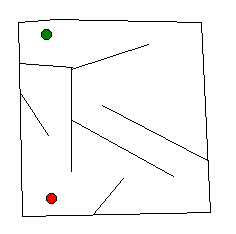
\includegraphics[width=.30\linewidth,height=.30\linewidth]{images/hard_maze}}~~~
    \subfigure{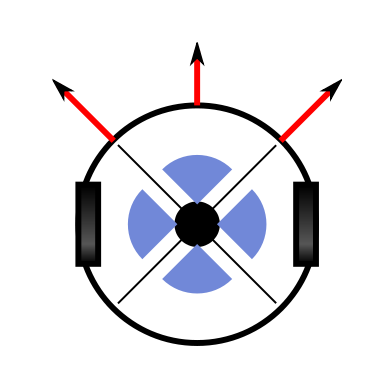
\includegraphics[width=.30\linewidth,height=.30\linewidth]{images/robot}}~~~
    \subfigure{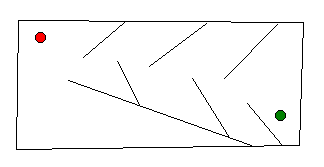
\includegraphics[width=.30\linewidth,height=.30\linewidth]{images/medium_maze}}
\end{figure}
\end{frame}


\begin{frame}{Expériences}
\begin{block}{Critères}
    \begin{enumerate}
        \item fitness = distance au point d'arrivé à un temps t
        \item nouveauté = densité autour de la position finale du robot à un temps t
    \end{enumerate}
\end{block}
\end{frame}


\begin{frame}
\frametitle{NoveltySearch C++}
Prise en main de la plate-forme \emph{NoveltySearch C++}
\begin{itemize}
    \item écriture d'outils pour visualiser et étudier le fonctionnement de la plate-forme
    \begin{itemize}
        \item MapViewer : affiche les labyrinthes (en C++/Qt) avec les résultats
        \item MazeViewer : affiche les labyrinthes (en Python/PySFML)
        \item NNViewer : affiche les réseaux de neurones (en C++/Qt)
    \end{itemize}
    \item modification de la plate-forme
    \begin{itemize}
        \item agrégation fitness et nouveauté
        \item tracé des individus dans le labyrinthe
        \item de nombreuses autres petites modifications (hooks, ...)
    \end{itemize}
    \item écriture de scripts pour visualiser les résultats
    \begin{itemize}
        \item plusieurs scripts (octave, python, ruby, shell)
        \item des vidéos montrant la progression de l'évolution
    \end{itemize}
\end{itemize}
\end{frame}


\begin{frame}{Outils et scripts}
%\begin{figure}
%    \centering
%    \subfigure{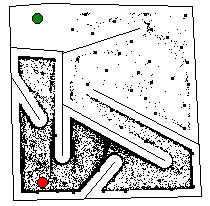
\includegraphics[width=.40\linewidth,height=.30\linewidth]{images/hard_nov}}~~~
%    \subfigure{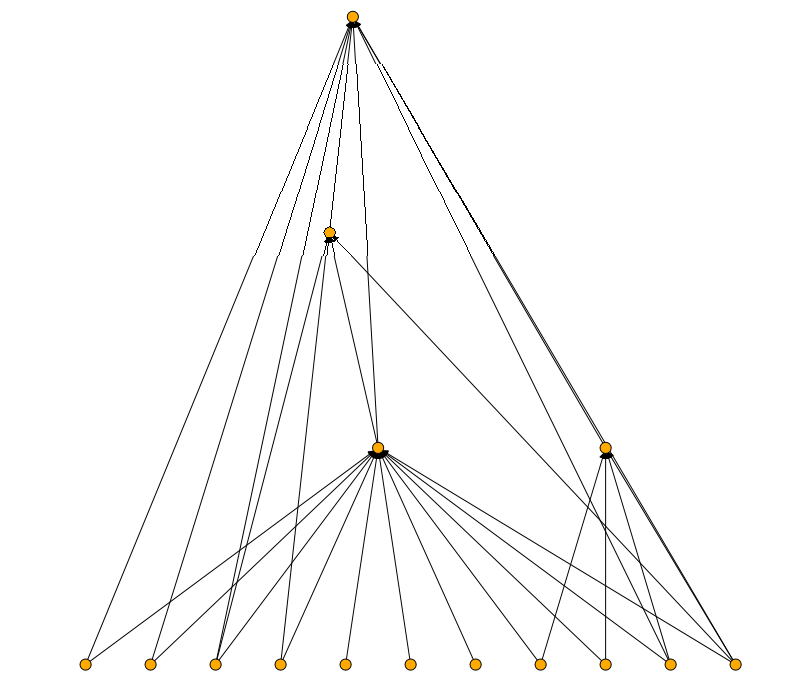
\includegraphics[width=.40\linewidth,height=.30\linewidth]{images/nnv1}}
%\end{figure}
\begin{center}
    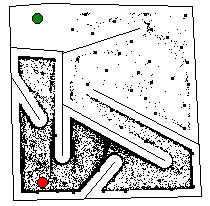
\includegraphics[width=.65\linewidth]{images/hard_nov}
\end{center}
\end{frame}


\begin{frame}{Outils et scripts}
\begin{center}
    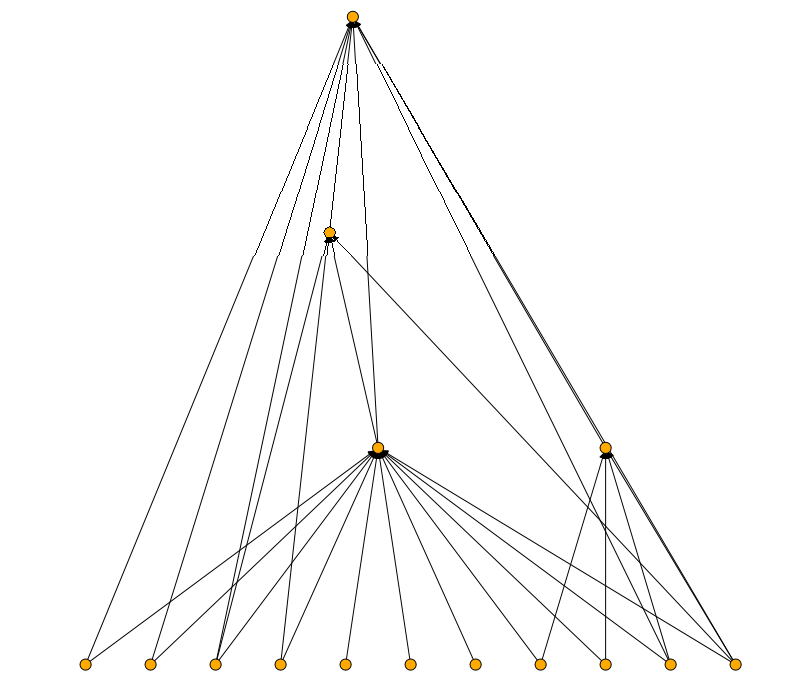
\includegraphics[width=.75\linewidth]{images/nnv1}
\end{center}
\end{frame}


\begin{frame}{Outils et scripts}
\begin{center}
    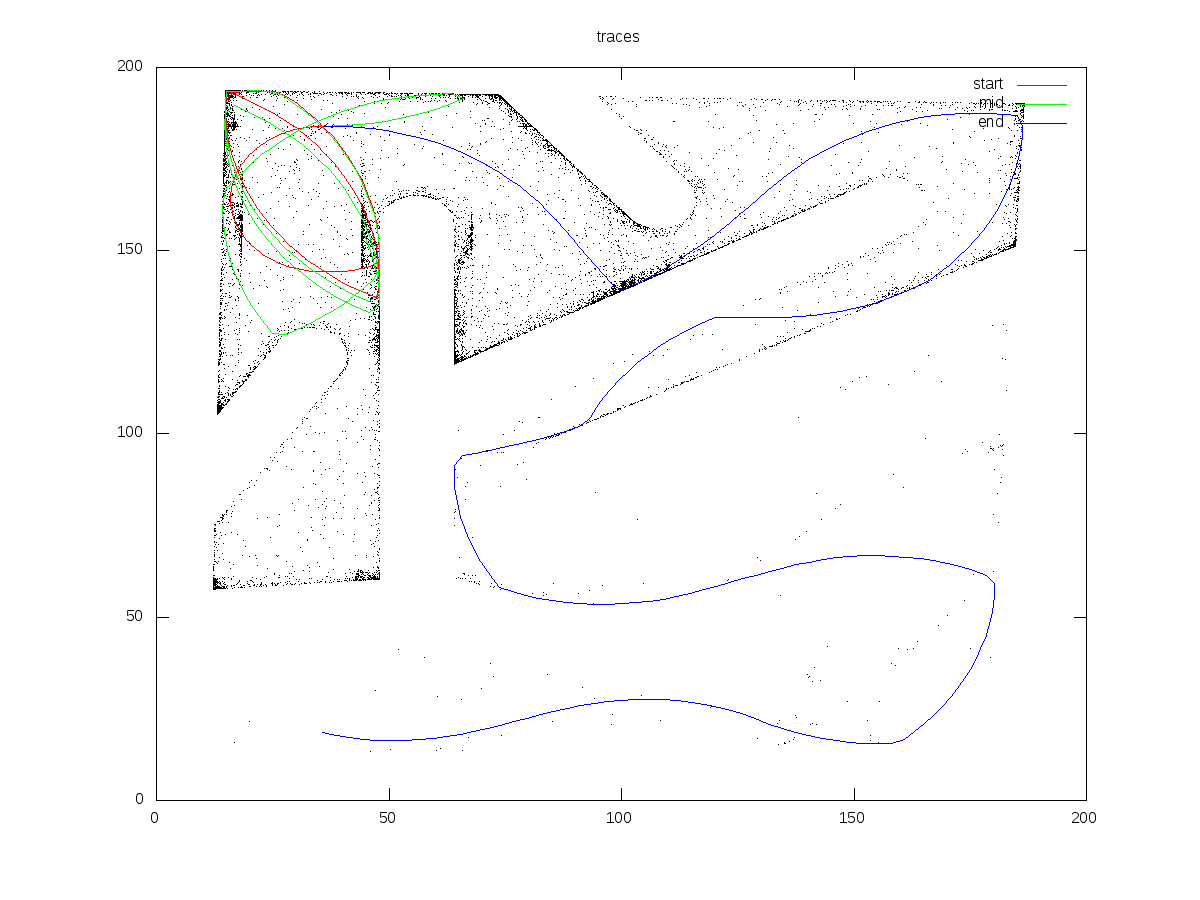
\includegraphics[width=.95\linewidth]{images/traces}
\end{center}
\end{frame}


\begin{frame}{Outils et scripts}
\begin{figure}
    \centering
    \subfigure{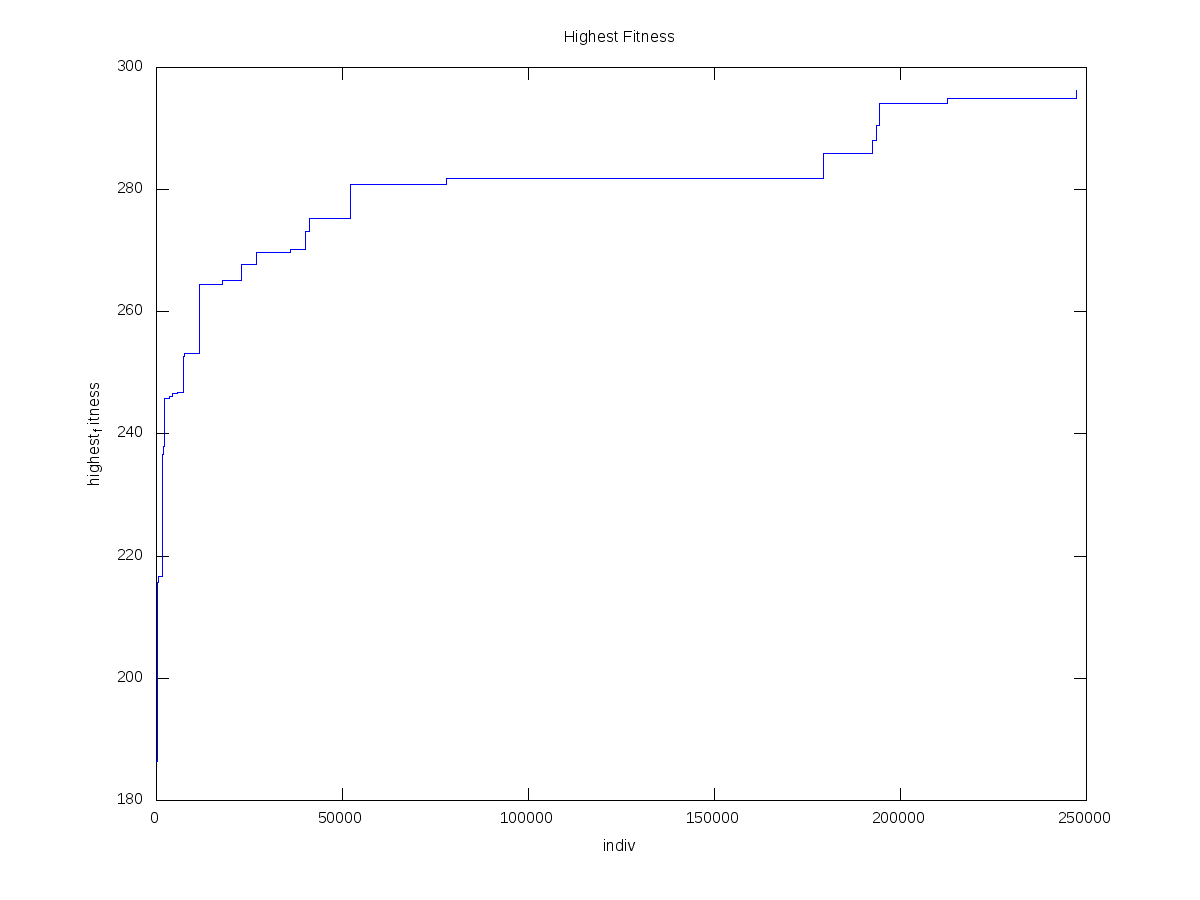
\includegraphics[width=.30\linewidth,height=.30\linewidth]{images/snail2_nov}}~~~
    \subfigure{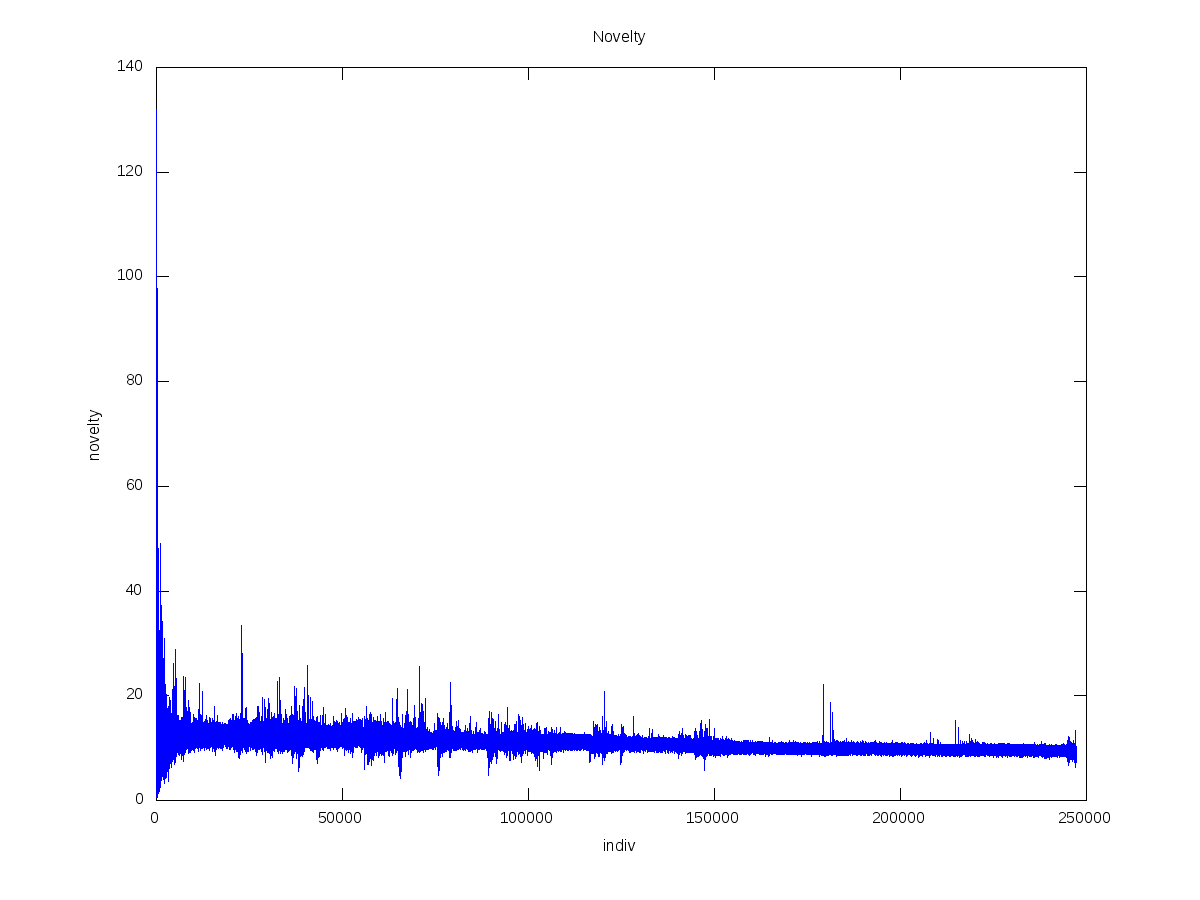
\includegraphics[width=.30\linewidth,height=.30\linewidth]{images/novelty}}~~~
    \subfigure{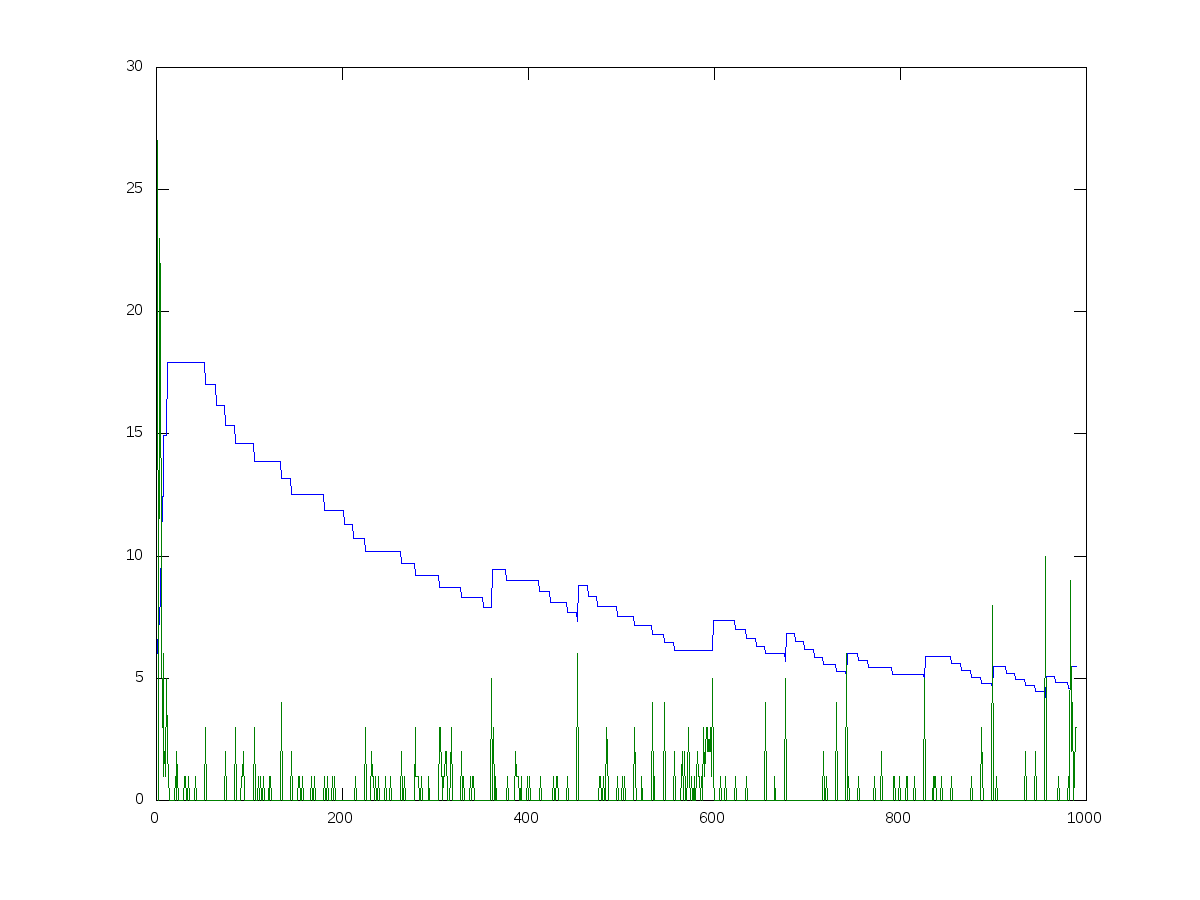
\includegraphics[width=.30\linewidth,height=.30\linewidth]{images/runresults}}
\end{figure}
\end{frame}


\subsection{Expériences initiales}

\begin{frame}{Plan - \secname}
\tableofcontents[sectionstyle=hide/hide,subsectionstyle=show/shaded/hide ]
\end{frame}


\begin{frame}
\frametitle{Vérification des expériences}
Vérification des expériences de l'article
\begin{itemize}
    \item Fitness (moyenne sur 5 run)
    \item Novelty (moyenne sur 5 run)
\end{itemize}
\begin{figure}
    \centering
    \subfigure{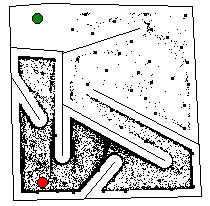
\includegraphics[width=.40\linewidth,height=.30\linewidth]{images/hard_nov}}~~~
    \subfigure{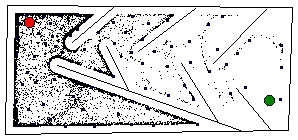
\includegraphics[width=.40\linewidth,height=.30\linewidth]{images/medium_nov}}
\end{figure}
\end{frame}


\begin{frame}{Résultats}
Medium maze (moyenne sur 5 run)
\begin{center}
    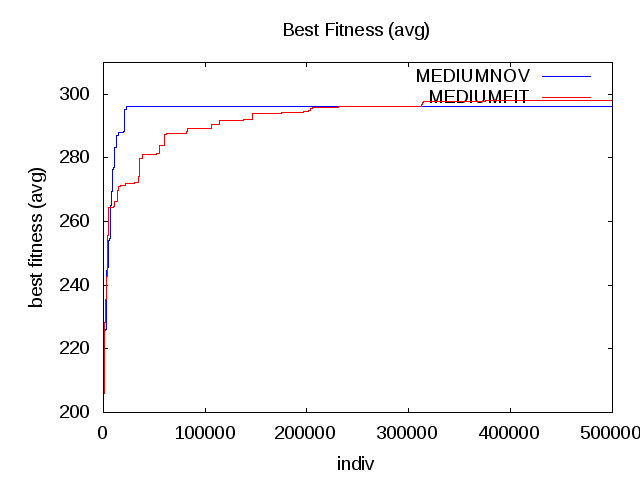
\includegraphics[width=.95\linewidth]{images/medium_bestfitness_means}
\end{center}
\end{frame}


\begin{frame}{Résultats}
Hard maze (moyenne sur 5 run)
\begin{center}
    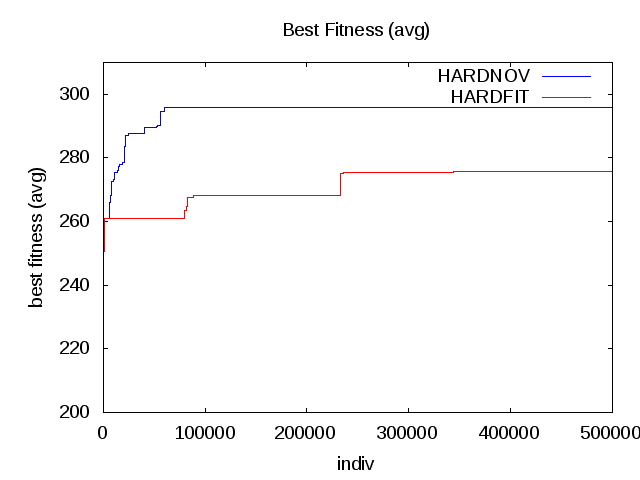
\includegraphics[width=.95\linewidth]{images/hard_bestfitness_means_1}
\end{center}
\end{frame}


\begin{frame}{Résultats}
Les résultats sont comparables à ceux de Lehman et Stanley
\begin{itemize}
    \item la fitness est piégée par la hardmap et ne parvient pas souvent à l'optimal
    \item la recherche de nouveauté converge toujours sur les deux cartes
    \item la recherche de nouveauté converge beaucoup plus vite qu'avec la fitness (quand elle y parvient)
\end{itemize}
~\\
On observe toutefois quelques différences
\begin{itemize}
    \item nos expériences convergent plus rapidement
    \item la recherche par fitness obtient des résultats légèrement supérieurs
\end{itemize}
~\\
Nous utilisons pourtant les mêmes paramètres
\end{frame}


\subsection{Expériences supplémentaires}

\begin{frame}{Plan - \secname}
\tableofcontents[sectionstyle=hide/hide,subsectionstyle=show/shaded/hide ]
\end{frame}


\begin{frame}
\frametitle{Expériences supplémentaires}
Exploration de la méthode avec d'autres expériences
\begin{figure}
    \centering
    \subfigure{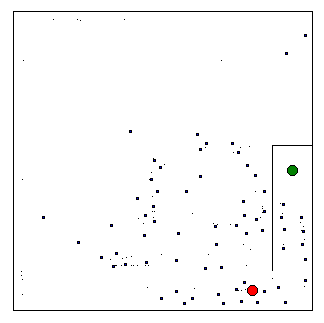
\includegraphics[width=.40\linewidth,height=.30\linewidth]{images/easy_nov}}~~~
    \subfigure{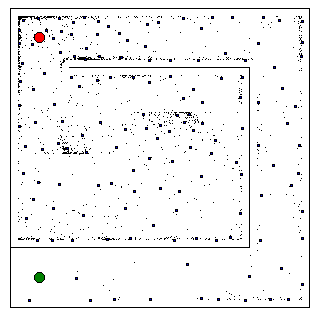
\includegraphics[width=.40\linewidth,height=.30\linewidth]{images/easysnail_nov}}
    ~\\
    \subfigure{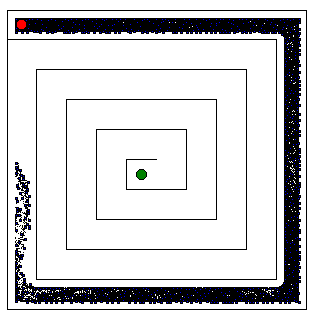
\includegraphics[width=.40\linewidth,height=.30\linewidth]{images/snail}}~~~
    \subfigure{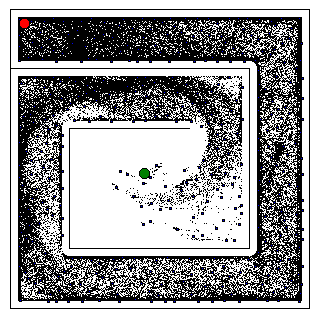
\includegraphics[width=.40\linewidth,height=.30\linewidth]{images/snail_nov}}
\end{figure}
\end{frame}


\begin{frame}{Outils et scripts}
\begin{figure}
    \centering
    \subfigure{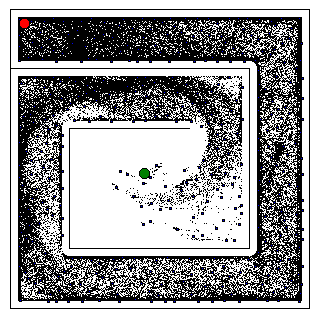
\includegraphics[width=.40\linewidth,height=.30\linewidth]{images/snail_nov}}~~~
    ~\\
    \subfigure{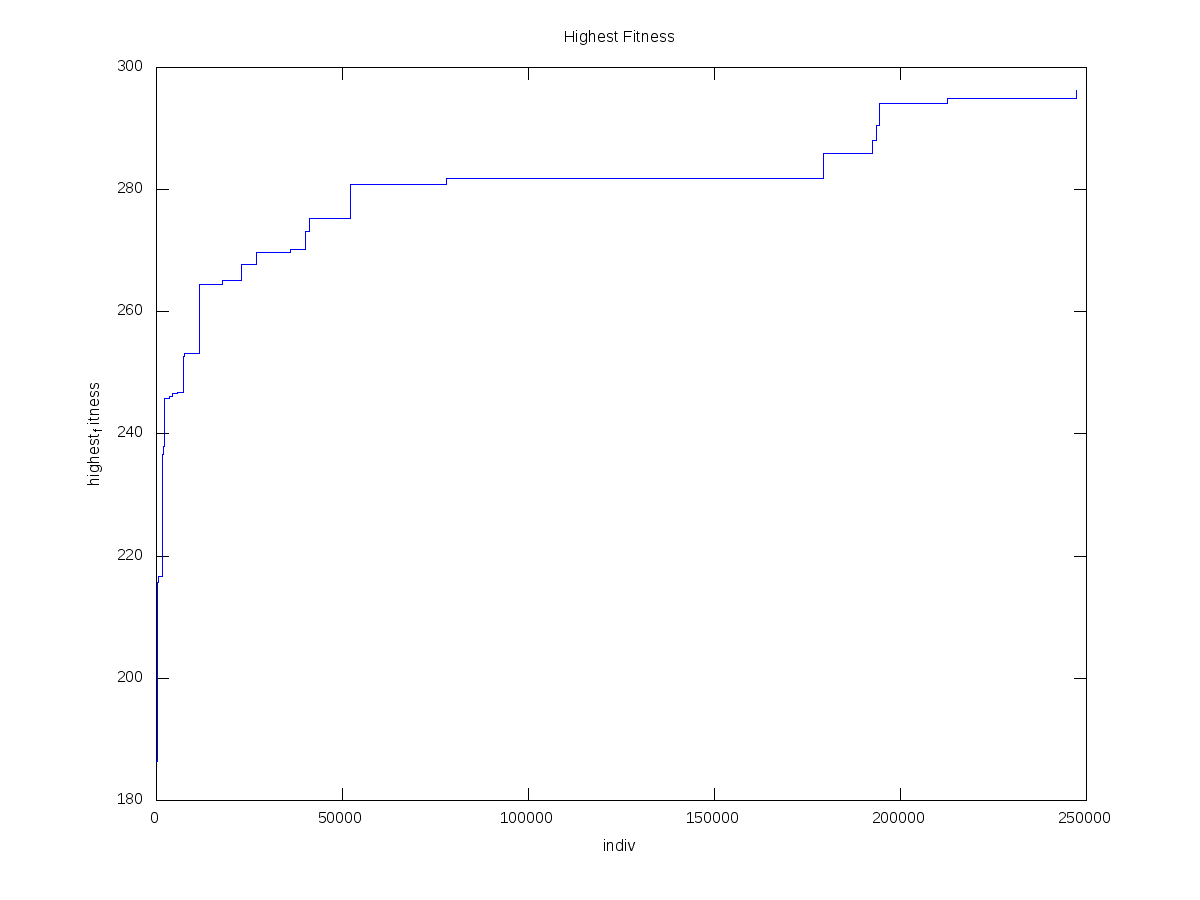
\includegraphics[width=.30\linewidth,height=.30\linewidth]{images/snail2_nov}}~~~
    \subfigure{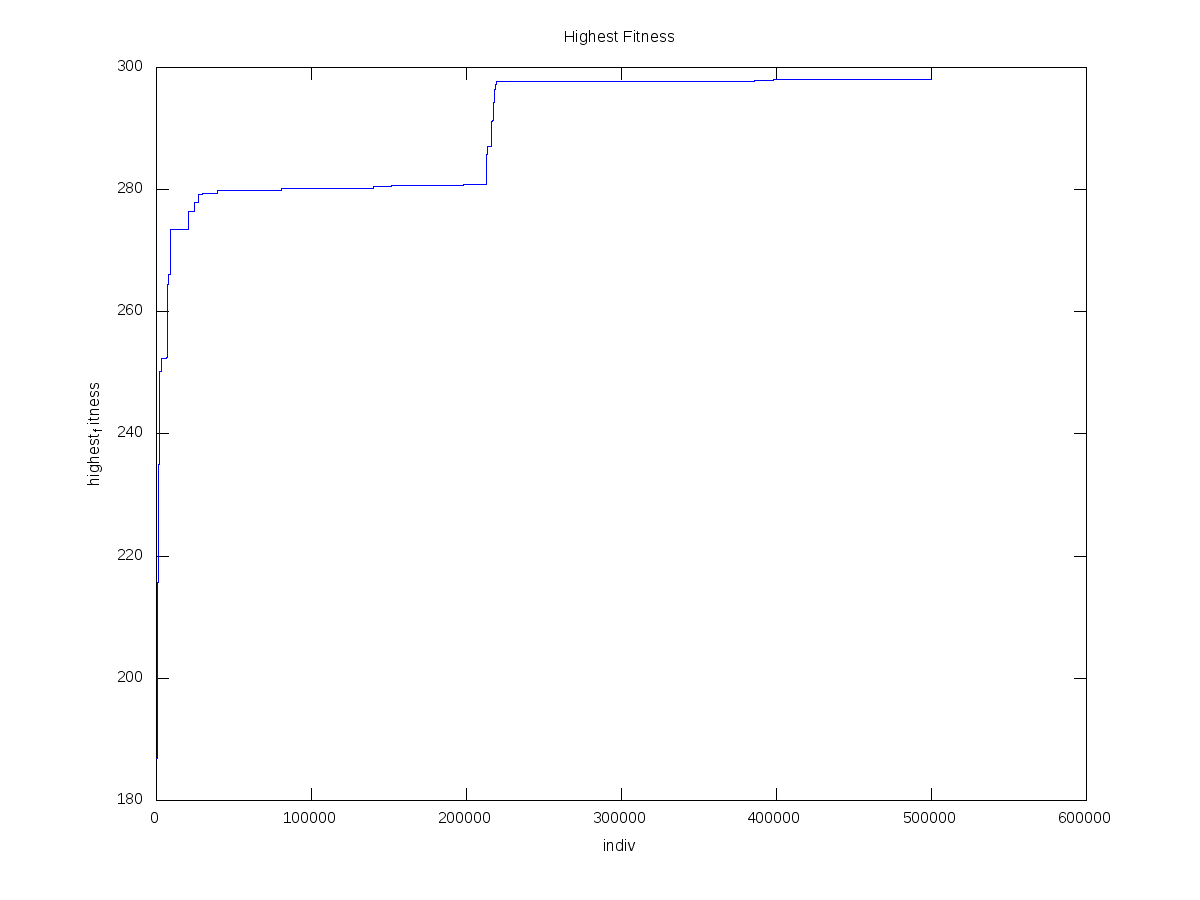
\includegraphics[width=.30\linewidth,height=.30\linewidth]{images/snail2_fit}}
\end{figure}
\end{frame}


\subsection{Extension de la méthode}

\begin{frame}{Plan - \secname}
\tableofcontents[sectionstyle=hide/hide,subsectionstyle=show/shaded/hide ]
\end{frame}


\begin{frame}{Fitness et nouveauté}
	Nous avons testé plusieurs fonctions d'agrégation :
	\begin{block}{La combinaison linéaire}
		$$\alpha*fitness + (1 - \alpha)*novelty$$
	\end{block}
	\begin{block}{La combinaison probabiliste}
		$$fitness * novelty$$
	\end{block}
	\begin{block}{La combinaison linéaire en fonction du temps}
		$$\alpha(t)*fitness + (1 - \alpha(t))*novelty$$
		\begin{enumerate}
			\item exponentielle	$\alpha(t) = \exp^{t - T_{max}}$
			\item sinusoïdale $\alpha(t) = 0.5+\sigma*sin(\frac{t}{\tau})$
		\end{enumerate}
	\end{block}
\end{frame}


\begin{frame}{Résultats}
La combinaison linéaire (moyenne sur 5 run)
\begin{center}
    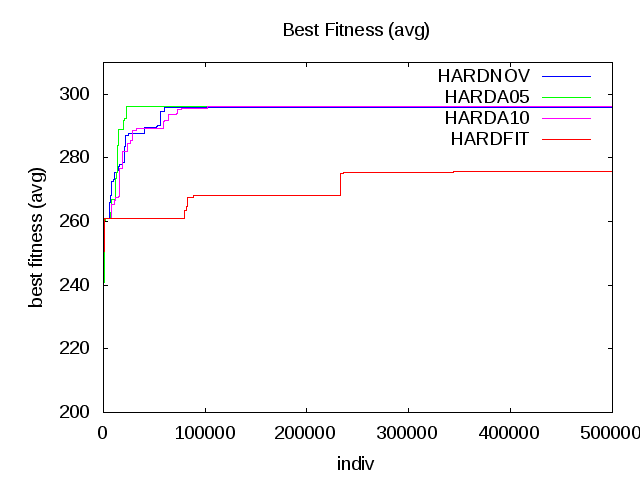
\includegraphics[width=.95\linewidth]{images/hard_bestfitness_means}
\end{center}
\end{frame}


%\begin{frame}{Résultats}   % TODO
%La combinaison probabiliste
%La combinaison linéaire en fonction du temps
%IMAGES ...
%\end{frame}

%%%%%%%%%%%%%%%%%%%%%%%%%%%%%%%%%%%%%%%

\section{Discussion et conclusion}
\begin{frame}
\begin{center}
{\LARGE Discussion et conclusion}
\end{center}
\end{frame}


\subsection{Conclusion}

\begin{frame}
\frametitle{Conclusion}
Résultats
\begin{itemize}
    \item les résultats sont conformes aux attentes
    \item la recherche par nouveauté contourne les limites des méthodes traditionnelles
\end{itemize}
~\\
Retombées
\begin{itemize}
    \item la recherche par nouveauté est une approche originale et très prometteuse pour améliorer les performances des algorithmes évolutionnistes
    \item des travaux récents ont montrés qu'elle améliore significativement les performances les réseaux de neurones adaptatifs [Risi and al., 2009]
\end{itemize}
\end{frame}


\begin{frame}
\frametitle{Discussion}
\begin{itemize}
    \item la recherche par nouveauté supprime un point délicat : la recherche d'une fonction de fitness efficace (bootstrap, etc.)...
    \item mais il faut toutefois choisir une bonne mesure de distance dans l'espace de recherche (point final, chemin, ...)
\end{itemize}
~\\
\begin{itemize}
    \item nous avons également montré qu'une approche moins radicale que celle proposée par Lehman et Stanley offre de meilleurs résultats
    \item toutefois l'agrégation n'est pas une solution idéale (solutions ignorées, ...)
    \item la multiobjectivisation basée sur l'algorithme MOEA offre de meilleures performances [Mouret, 2009]
\end{itemize}
\end{frame}


%%%%%%%%%%%%%%%%%%%%%%%%%%%%%%%%%%%%%%%

\begin{frame}[allowframebreaks]
\frametitle{Bibliographie}
\begin{itemize}
    \item $[$Lehman and Stanley, 2008$]$
    J.~Lehman and K.O. Stanley.
    Exploiting open-endedness to solve problems through the search for
    novelty.
    In  Proceedings of the Eleventh International Conference on
    Artificial Life (ALIFE XI) Cambridge MA: MIT Press, volume~54, 2008.

    \item $[$Mouret, 2009$]$
    J.B. Mouret.
    Novelty-based multiobjectivization.
    In  Proceedings of IROS Workshop” Exploring New Horizons in the
    Evolutionary Design of Robots, 2009.

    \item $[$Mouret and Doncieux, 2008$]$
    J.B. Mouret and S.~Doncieux.
    Incremental evolution of animats' behaviors as a multi-objective
    optimization.
    Lecture Notes in Computer Science, 5040:210--219, 2008.

    \item $[$Mouret and Doncieux, 2009$]$
    J.B. Mouret and S.~Doncieux.
    Overcoming the bootstrap problem in evolutionary robotics using
    behavioral diversity.
    In  Proceedings of the Congress on Evolutionary Computation 2009
    (to appear), 2009.

    \item $[$Risi and al., 2009$]$
    S.~Risi, S.D. Vanderbleek, C.E. Hughes, and K.O. Stanley.
    How novelty search escapes the deceptive trap of learning to learn.
    In  Proceedings of the 11th Annual conference on Genetic and
    evolutionary computation, pages 153--160. ACM, 2009.

    \item $[$Stanley, Bryant and Miikkulainen, 2005$]$
    K.O. Stanley, B.D. Bryant, and R.~Miikkulainen.
    Real-time neuroevolution in the NERO video game.
    IEEE Transactions on Evolutionary Computation, 9(6):653--668,
    2005.

    \item $[$Stanley and Miikkulainen, 2002$]$
    K.O. Stanley and R.~Miikkulainen.
    Evolving neural networks through augmenting topologies.
    Evolutionary Computation, 10(2):99--127, 2002.

    \item $[$Stanley and Miikkulainen, 2004$]$
    K.O. Stanley and R.~Miikkulainen.
    Competitive coevolution through evolutionary complexification.
    Journal of Artificial Intelligence Research, 21(1):63--100,
    2004.

%    \item $[$9$]$
%    S.~Koos, J.B. Mouret, and S.~Doncieux.
%    Automatic system identification based on coevolution of models and
%    tests.
%    In  IEEE Congress on Evolutionary Computation, volume 2009,
%    2009.
\end{itemize}
\end{frame}

\begin{frame}
\begin{center}
    \href{http://creativecommons.org/licenses/by-sa/2.0/fr/}{
\includegraphics[width=.40\linewidth]{images/cc_by_sa}}
    %\\[3em]
    %\textbf{Illustrations}\\\medskip
    %\href{http://commons.wikimedia.org/wiki/User:Nojhan}{Johann "nojhan" Dréo} \raisebox{-0.5\height+0.3em}{\href{http://creativecommons.org/licenses/by-sa/2.0/fr/}{
\includegraphics[height=1em]{images/cc_by_sa_small}}}
\end{center}
\end{frame}

\end{document}
